\documentclass{article}
\usepackage{hyperref}
\usepackage{graphicx}
\usepackage{caption}
\usepackage{subcaption}
\begin{document}
\title{`Continuous-Time' Synthesis and the Context of Timelab'}
\maketitle
\section{Introduction}

\subsection{why timelab?}
\subsubsection{issues with existing systems}

\paragraph{Music-N/CSound (Max Mathews and John ffitch, 1957-present)}
A classic programming environment, stemming from the pioneering work of Max Mathews, it is  widely used, and highly developed.
\begin{itemize}
\item rigid structure 
\item difficult to interact with / compile time
\item obtuse representation of scores and synths / hard to read: \href{./score.sco.html}{score} \href{./orc.html}{instrument}
\item score/instrument layout insists on antique perception of music composition/creation -- a notion which in many ways goes against the grain of analog electronic music practices 
  %note -- discuss Stockhausen, Shaffer, and Buchla here
\end{itemize} 

\paragraph{Max/Msp and Pd (David Zicarelli and Miller Puckette, 1987-present)}
An almost ubiquitous and highly interactive paradigm, these programs the are industry standards (commercial and open source respectively) for experimental audio algorithm design.
\begin{itemize}
\item patch chords and guis!!!%picture
\item difficulty of iterating loops%picture
\item difficulty in doing things in mass
\item flow diagram structure (borrowing from analog synthesizers) also insists on a way of thinking about music composition -- denying the user a `code-ish' mindset
\end{itemize}

\paragraph{SuperCollider (James McCartney, 1996-present)}
SC provides the interactiveness of Pd with the `codiness' of a text based programming environment such as CSound.
\begin{itemize}
\item server/client structure has benefits but designates a .2s default latency between server time and client time%McCartney lecture
\item non-standard editor and gui environments 
\end{itemize}

\paragraph{ChucK (Ge Wang and Perry Cook)}
ChucK is another text-based audio programming environment that emphasizes a live-coding ethos. 
\begin{itemize}
\item admittedly emphasizes ease of programming over performance (ChucK is slow)
\item unintuitive approach to time by treating `now' as a variable that we manipulate by hand: \url{http://en.wikipedia.org/wiki/ChucK}
\end{itemize}

\subsubsection{Fall 2012 206}
\subsubsection{Control timing}
All of the above metnioned systems have specific solutions to problems of rectifying the timing between control input and precisely when control is enacted in the DSP engine. Cf. my poster from last year's ICMC (TIMELAB: YET, YET ANOTHER REAL-TIME AUDIO PROGRAMMING SYSTEM -- not yet available online) for a quick and dirty on this subject.

Also of relevance are these talks by Miller Puckette and James McCartney:
\url{http://repmus.ircam.fr/mutant/rtmseminars}
\begin{itemize}
\item Puckette talk: 9:30 - 15:00 : DAGs and mutual exclusion, determinism
\item McCartney talk: 29:00 - 37:45 : control rate issues
\end{itemize}

\subsubsection{embedded audio programming}
Just the other day (Friday, March 14) someone posted to the Pd-list asking if it was possible to crunch a Pd patch down into a guitar pedal (the answer was `no, not really'). Clearly, there is a market for throwing these kinds of experimental algorithms into a guitar pedal packages. One solution is to utilize micro computers such as the Raspberry Pi or UDOO. Another is to have an audio programming API in C with a build environment that can target truly embedable hardware, such as ST's discovery board featuring the ARM Cortex processor (or any of the open source solutions built around these chips).

\section{Continuous-Time Synthesis}
\paragraph{What is meant by `continuous-time synthesis'}
\begin{itemize}
\item as distinct from traditional computer music DSP structure which consists of UGens and signal flow
\item uses differential equations to model synthesis behaviors
\item create complex synthesis algorithms by arranging equations in a network with interleaved numerical solver stages so that time does not pass between nodes in the network
\end{itemize}
This affords us advantages that are beyond the scope of UGen/signal flow structures.
\subsection{0-time delay lines}
The object of allowing for 0-time delay lines in a network is to fascilitate (among other things) accurate sync-ing. In the parlance of analog synthesizers, a master oscillator may slave another one to it by resetting the phase of the slave at every other zero crossing (period) of the master. 
\begin{figure}
  \centering
  
  \begin{subfigure}[b]{0.3\textwidth}
    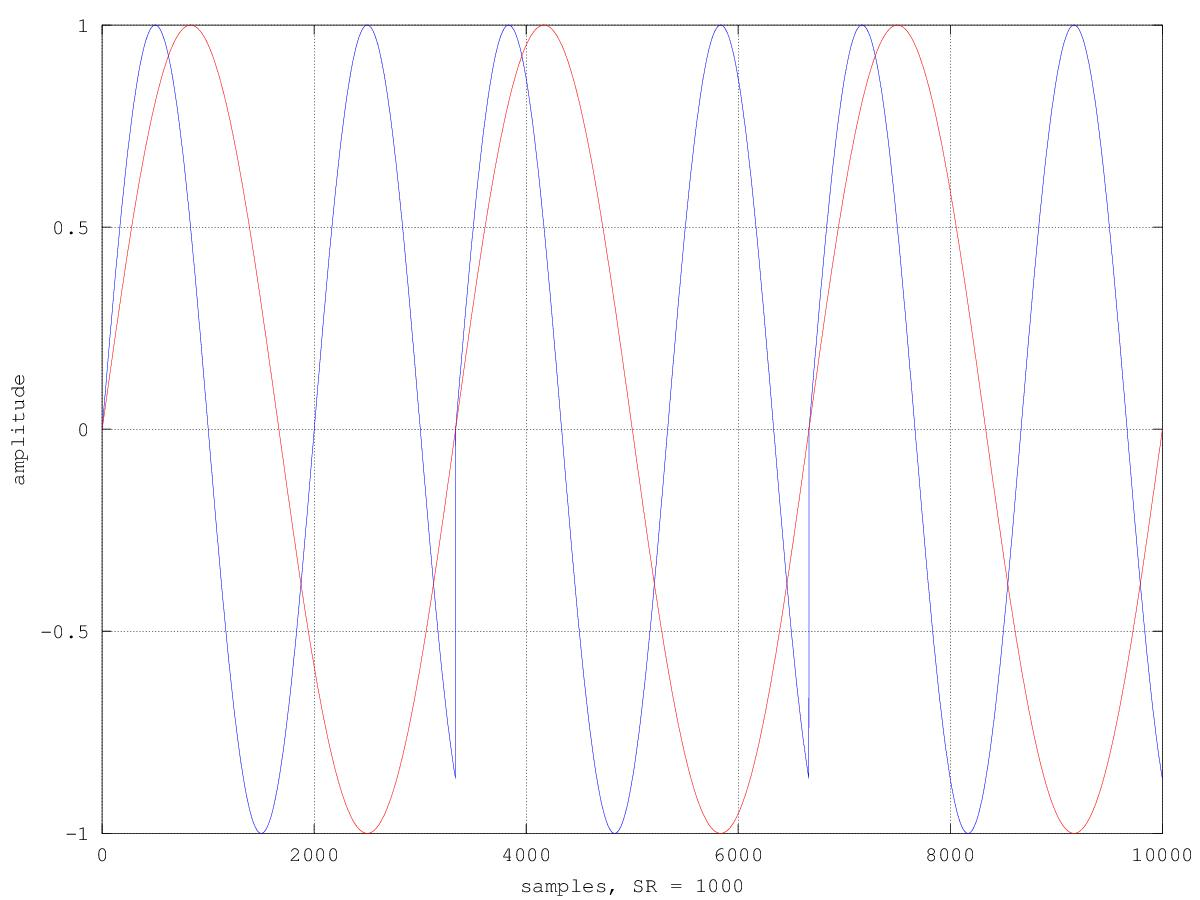
\includegraphics[width=3in]{sync4}
    \caption{red syncs blue}
  \end{subfigure}
  
  \begin{subfigure}[b]{0.3\textwidth}
    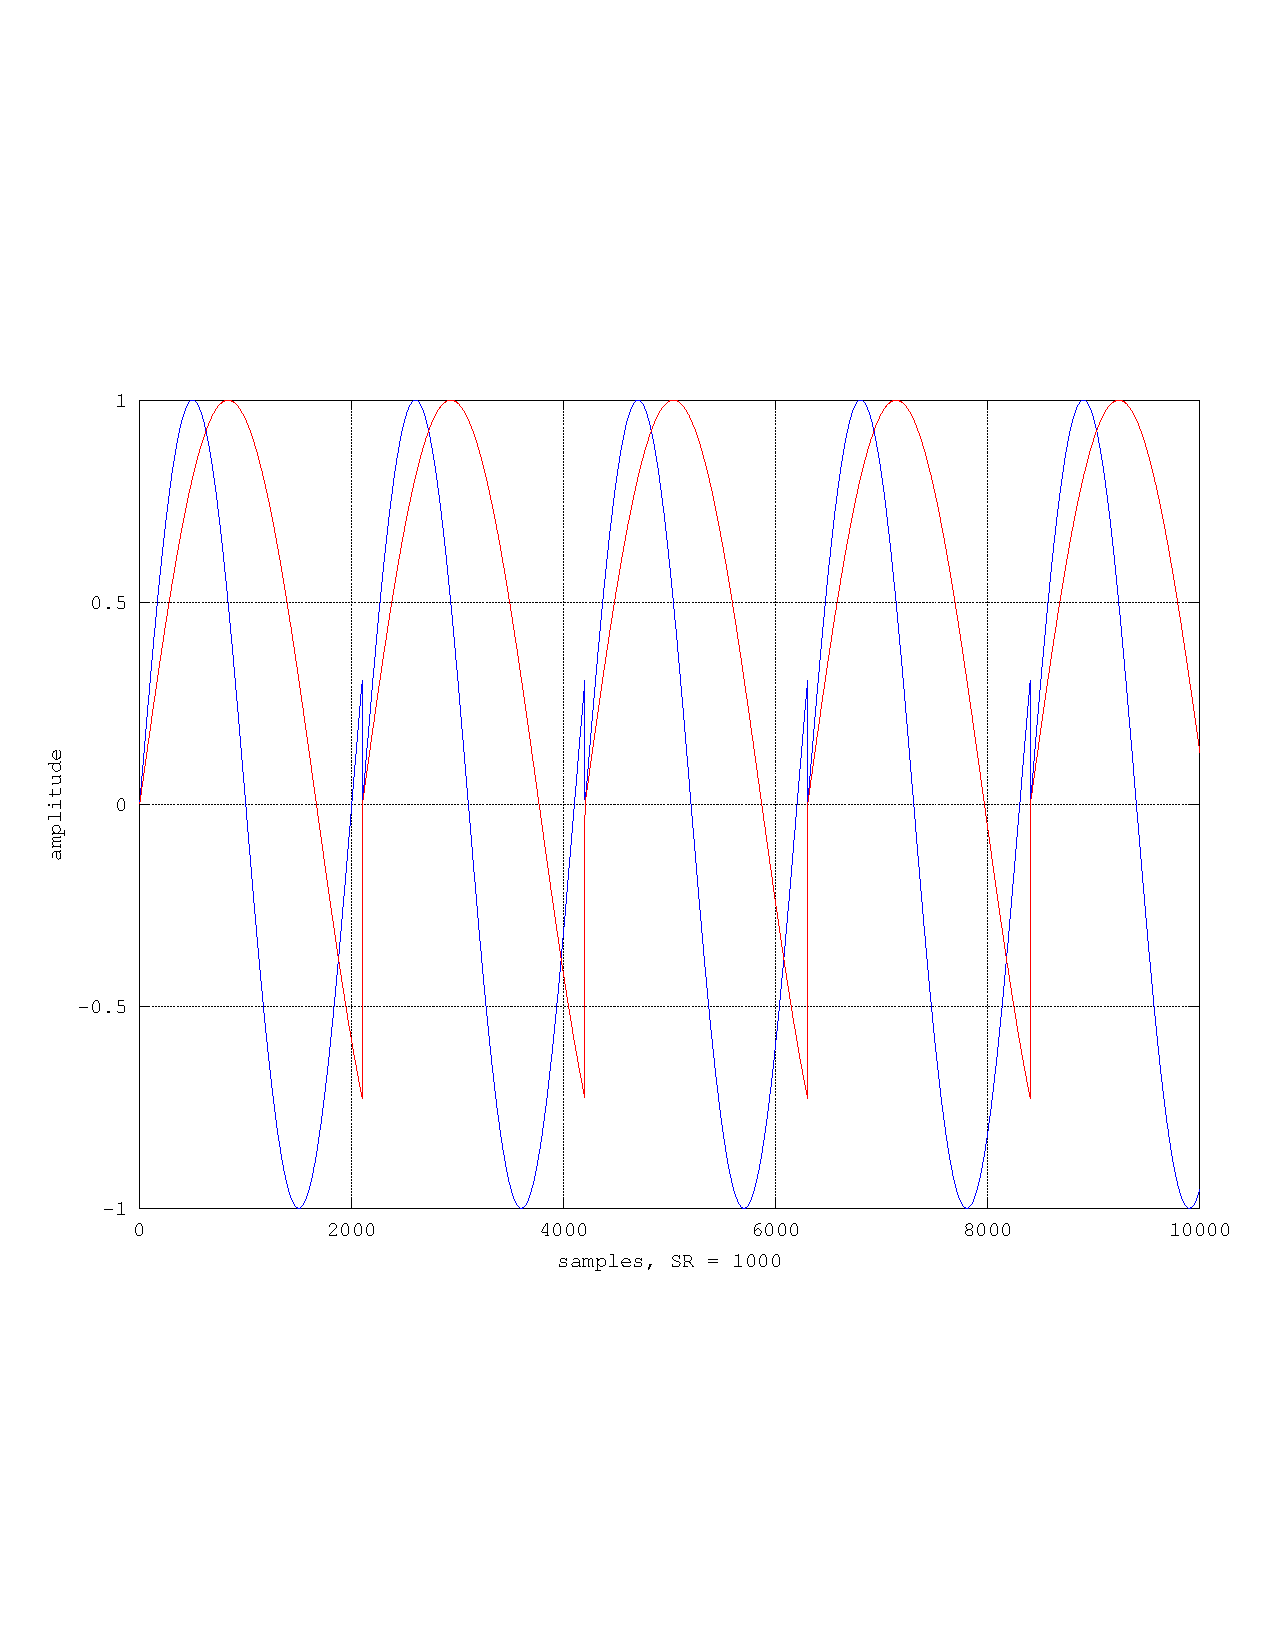
\includegraphics[width=3in]{sync6}
    \caption{misaligned sync}
  \end{subfigure}
  \label{fig-syncs}\caption{On the left, the blue oscillator is slaved to the red. On the right each is slaved to the other, but notice the `hiccups' due to non-zero-time delay betwen the oscillators.}
\end{figure}
\subsection{virtual analog}
\subsubsection{ngspice}
\subsubsection{wave-digital filters}
\subsubsection{quadrature oscillator}
\subsubsection{moog filter example}

\subsection{new models for new sounds}
\subsubsection{noisey oscillators}
%examples -- applications (lfos) do a patch
\subsubsection{non-linear filters}
%????
\subsubsection{a new way to view synthesis}

\subsection{What's Next?}
%control, more features
\section{Timelab}
\subsection{Brief Overview}
\subsection{Examples}
\end{document}
